%% Erläuterungen zu den Befehlen erfolgen unter
%% diesem Beispiel.

\documentclass{scrartcl}

\usepackage[utf8]{inputenc}
\usepackage[T1]{fontenc}
\usepackage{lmodern}
\usepackage[ngerman]{babel}
\usepackage{amsmath}
\usepackage{graphicx}

\title{Der Eventmanager mit Wetter und Events}
\author{\underline{Maximilian von Hohenbühel}, Alex Moroder}
\date{19. Februar 2020}
\begin{document}

\maketitle
\tableofcontents
\section{Einleitung}

Diese Webapplikation ist eine Erweiterung von unserem alten TP-Projekt. 
Beim alten TP-Project konnte man sich anmelden, Termine erstellen mit einem Datum, Name und Zeitpunkt und neue Nutzer anlegen.
Wir haben uns nach Fertigstellung des alten Projekts gedacht, dass wenn wir schon Termine anlegen, dann wäre es fein, 
    wenn der Nutzer auch gleich weis, was er an bestimmten Uhrzeiten und Orten machen kann. Dazu gibt es auch die Möglichkeit 
    sich das Wetter von ganz Südtirol anzeigen zu Lassen und Daten von bestimmten Orten.

    \section{Technologien}

    \subsection{Backend}

    Das Backend ist für die Verarbeitung der Daten und für den Server zustandig.

    \subsubsection{NodeJs}

    Wir verwenden NodeJs, gezielt den ExpressJs Server um unser Projekt zu hosten.
    NodeJs ist eine JavaScript-Laufzeitumgebung, die eine \textbf{geringe Latenz} und einen \textbf{hohen Durchsatz} erzielt, 
    indem Anforderungen nicht blockiert werden Abb:\ref{fig:node}.
    \begin{figure}[h]
    \centering
    
\includegraphics{"~/Documents/TP/DeWeis/DeWeisClient/src/assets/images/node_express.jpg"}
    \caption{NodeJs - Logo}
    \label{fig:node}
    \end{figure}

    \subsubsection{MariaDB}


    MariaDB ist eine der popularsten Datenbanksysteme und ist für seine \textbf{Leistung, Stabilität, and Offenheit} bekannt.
    Wir haben uns dafur entschieden, da sie frei verfügbar ist, einfach zu implementieren und schnell mit unseren Daten umgehen kann.
    Wir benutzen die Datenbank hauptsachlich für das Speichern unserer Nutzer und deren Termine. In der zukunft konnte man ausserdem,jedem 
    Termin einen Ort geben und so auch die passenden Wetterdaten und Ortsinformationen in der Datenbank speichern Abb:\ref{fig:maria}.
    \begin{figure}[h]
    \centering
    \includegraphics{"~/Documents/TP/DeWeis/DeWeisClient/src/assets/images/mariadb"}
    \caption{MariaDB - Logo}
    \label{fig:maria}
    \end{figure}


    \subsubsection{OpenDataHub}

    Wir haben zum erhalten der Wetterdaten und Ortsangaben den OpenDataHub von Südtirol benutzt Abb:\ref{fig:open}.
    \begin{figure}[h]
    \centering
    \includegraphics{"~/Documents/TP/DeWeis/DeWeisClient/src/assets/images/opendatahub"}
    \caption{OpenDataHub - Logo}
    \label{fig:open}
    \end{figure}

    \subsection{Frontend}

    Das Frontend wird dazu verwendet die verarbeiteten Daten anzuzeigen und Input vom Nutzer an das Backend weiterzugeben.

    \subsubsection{Angular - Material}

    Angular Material hilft dabei, Daten schön und einfach auszugeben. Wir benutzen es im speziellen für die Knöpfe 
    und die Navigationsleiste. Die Timeline für die Termine ist auch mit den Material vorgaben gelöst Abb:\ref{fig:mat}.
    \begin{figure}
    \centering
    
\includegraphics{"~/Documents/TP/DeWeis/DeWeisClient/src/assets/images/material.png"}
    \caption{Angular-Material - Logo}
    \label{fig:mat}
    \end{figure}

    \subsubsection{Angular - Bootstrap}

    Angular Bootstrap ist wie Angular Material eine einfache Implementierung um Daten schön auszugeben. Wir benutzen Bootstrap 
    für das Bild Karussel des Wetters Abb:\ref{fig:boot}.
    \begin{figure}
    \centering
    \includegraphics{"~/Documents/TP/DeWeis/DeWeisClient/src/assets/images/index"}
    \caption{Angular-Bootstrap - Logo}
    \label{fig:boot}
    \end{figure}

    \subsubsection{Leaflet}

    Für die Anzeige der Karte haben wir uns für Leaflet und die Openstreetmap entschieden.
    Leaflet ist eine Open Source Implementierung für die Anzeige und Interaktion mit Karten.
    Wir benutzen sie um die Koordinaten des angeklickten Gebiets zu bekommen und sie danach weiterzuverarbeiten.
    Die Openstreetmap ist gut geeignet, da sie eine gute Indexierung bietet Abb:\ref{fig:leaf}.
    \begin{figure}
    \centering
    \includegraphics{"~/Documents/TP/DeWeis/DeWeisClient/src/assets/images/leaflet"}
    \caption{Leaflet - Logo}
    \label{fig:leaf}
    \end{figure}

    \section{Umsetzung}

    Wir haben begonnen indem wir uns mit den APIS auseinandergesetzt haben. Für die Daten in Südtirol haben wir die OpenDataHub - API 
    benutzt. Im speziellen die WetterAPI und die EnviromentAPI.

    \subsection{Probleme}

    Wir sind während unserer Arbeit auf kaum Probleme gestossen. Das größte Problem war dabei das Verstandnis des OpenDataHubs und 
    die Suche nach den richtigen Daten. Die unvollständigkeit des OpenDataHubs war auch eine große Hürde.

    \subsection{Erlerntes}

    Wir haben während unserer Arbeit viel über Südtirol und den OpenDataHub gelernt. Die Verwendung von Leaflet hat uns eine gute 
    Erkenntnis in die Benutzung von Karten gegeben und die Verarbeitung von Koordinaten.

    \subsection{Ablauf}

    Wir haben damit begonnen unser Projekt aufzuteilen, Alex Moroder macht den Eventmanager und Maximilian von Hohenbühel 
    macht die WetterAPI und die Ortsdaten. 

    \subsubsection{Eventmanager}

    Die einzelnen Punkte zur Vervollstandigung der Implementierung:
    \begin{enumerate}
    \item Recherche über die EventAPI vom OpenDataHub
    \item Implementierung einer Liste von möglichen Events Abb:\ref{fig:events}
    \begin{figure}[!h]
    \centering
    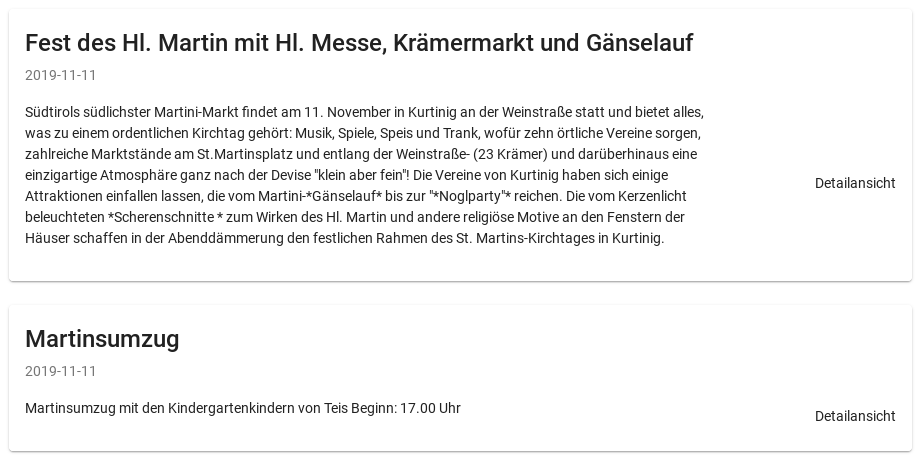
\includegraphics[scale=0.4]{"~/Documents/TP/DeWeis/DeWeisClient/src/assets/images/eventlist.png"}
    \caption{Liste von Events}
    \label{fig:events}
    \end{figure}
    \item Schreiben eines Suchfeldes um Interaktiv die Events zu finden Abb:\ref{fig:search}
    \begin{figure}[h]
    \centering
    
\includegraphics[scale=0.4]{"~/Documents/TP/DeWeis/DeWeisClient/src/assets/images/searchfield.png"}
    \caption{Suchfeld der Events}
    \label{fig:search}
    \end{figure}
    \item Ausgabe von näheren Informationen über ein Event beim Klick Abb:\ref{fig:detail}
    \begin{figure}[h]
    \centering
    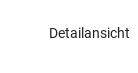
\includegraphics[scale=0.4]{"~/Documents/TP/DeWeis/DeWeisClient/src/assets/images/detail.png"}
    \caption{Knopf der Detailansicht}
    \label{fig:detail}
    \end{figure}
    \end{enumerate}

    \subsubsection{WetterAPI}

    Die einzelnen Punkte zur Vervollständigung der Implementierung:
    \begin{enumerate}
    \item WetterAPI des OpenDataHub durchsuchen und die wichtigen Daten herausschreiben
    \item Implementierung von Leaflet und die Suche nach der nächsten Wetterstation Abb:\ref{fig:map}
    \begin{figure}[h]
    \centering
    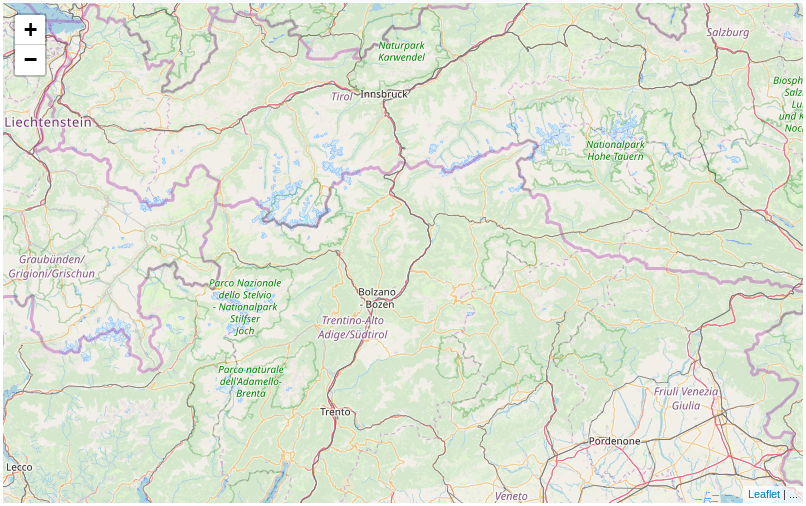
\includegraphics[scale=0.5]{"~/Documents/TP/DeWeis/DeWeisClient/src/assets/images/map.png"}
    \caption{Map}
    \label{fig:map}
    \end{figure}
    \item Ausgabe der wichtigsten Daten der Wetterstationen Abb:\ref{fig:weath}
    \begin{figure}[!h]
    \centering
    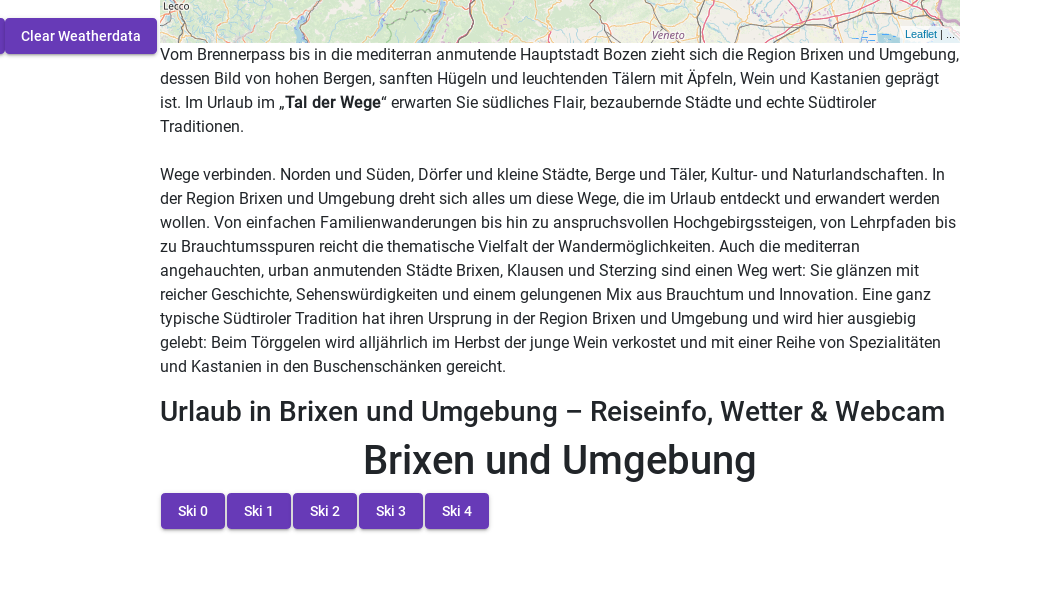
\includegraphics[scale=0.4]{"~/Documents/TP/DeWeis/DeWeisClient/src/assets/images/weatherinfo.png"}
    \caption{Daten der Wetterstation}
    \label{fig:weath}
    \end{figure}
    \item Ausgabe des Wetters von Südtirol mithilfe eines Karussels Abb:\ref{fig:caroussel}
    \begin{figure}[!h]
    \centering
    \includegraphics[scale=0.4]{"~/Documents/TP/DeWeis/DeWeisClient/src/assets/images/caroussel"}
    \caption{Karussel des Wetters}
    \label{fig:caroussel}
    \end{figure}
    \end{enumerate}

    \section{Quellen}
    \begin{itemize}
    \item[-] NodeJS -> https://nodejs.org/en/docs/
    \item[-] Leaflet -> https://github.com/Asymmetrik/ngx-leaflet
    \item[-] Bootstrap -> https://ng-bootstrap.github.io/\#/home
    \item[-] Material -> https://material.angular.io/
    \item[-] MariaDB -> https://mariadb.org/
    \item[-] OpenDataHub -> https://opendatahub.readthedocs.io/en/latest/index.html
    \item[-] Programmierfehler -> https://stackoverflow.com/
    \end{itemize}

    \end{document}
